\documentclass[border=2mm]{standalone}
\usepackage[utf8]{inputenc}
\usepackage[english]{babel}
\usepackage{tikz}
% \usepackage[margin=1cm]{geometry}
\usepackage[most]{tcolorbox}


\begin{document}
    \begin{tcolorbox}[
        colback=white, % Couleur de fond de la boîte
        colbacktitle=white, % Couleur de fond du titre de la boîte
        coltitle=black, % Couleur du titre de la boîte
        colframe=black, % Couleur du cadre de la boîte
        arc=2mm, % Rayon de l'arrondi des coins
        boxrule=2pt, % Épaisseur du cadre de la boîte
        % breakable, enhanced jigsaw,
        width=18cm,
        height=4.2cm,
        title=\LARGE \textbf{OFFLINE :} PINN training,
        halign title=center
        ]
        
        \centering
        \begin{tikzpicture}
            \draw[draw=black,dashed] (0,0) rectangle ++ (5,2.5);	
            \node at (2.5,1.85) {\Large \textbf{Inputs}};
            \node[anchor=west] at (0.1,1.1) {\large $\Omega$ : space domain};
            \node[anchor=west] at (0.1,0.5) {\large $\mathcal{M}$ : parameter domain};
            
            \draw[->, black, line width=2pt] (5.5,1.25) -- (6.5,1.25);
            
            \node[draw=none, inner sep=0pt] at (8.5,1.55) {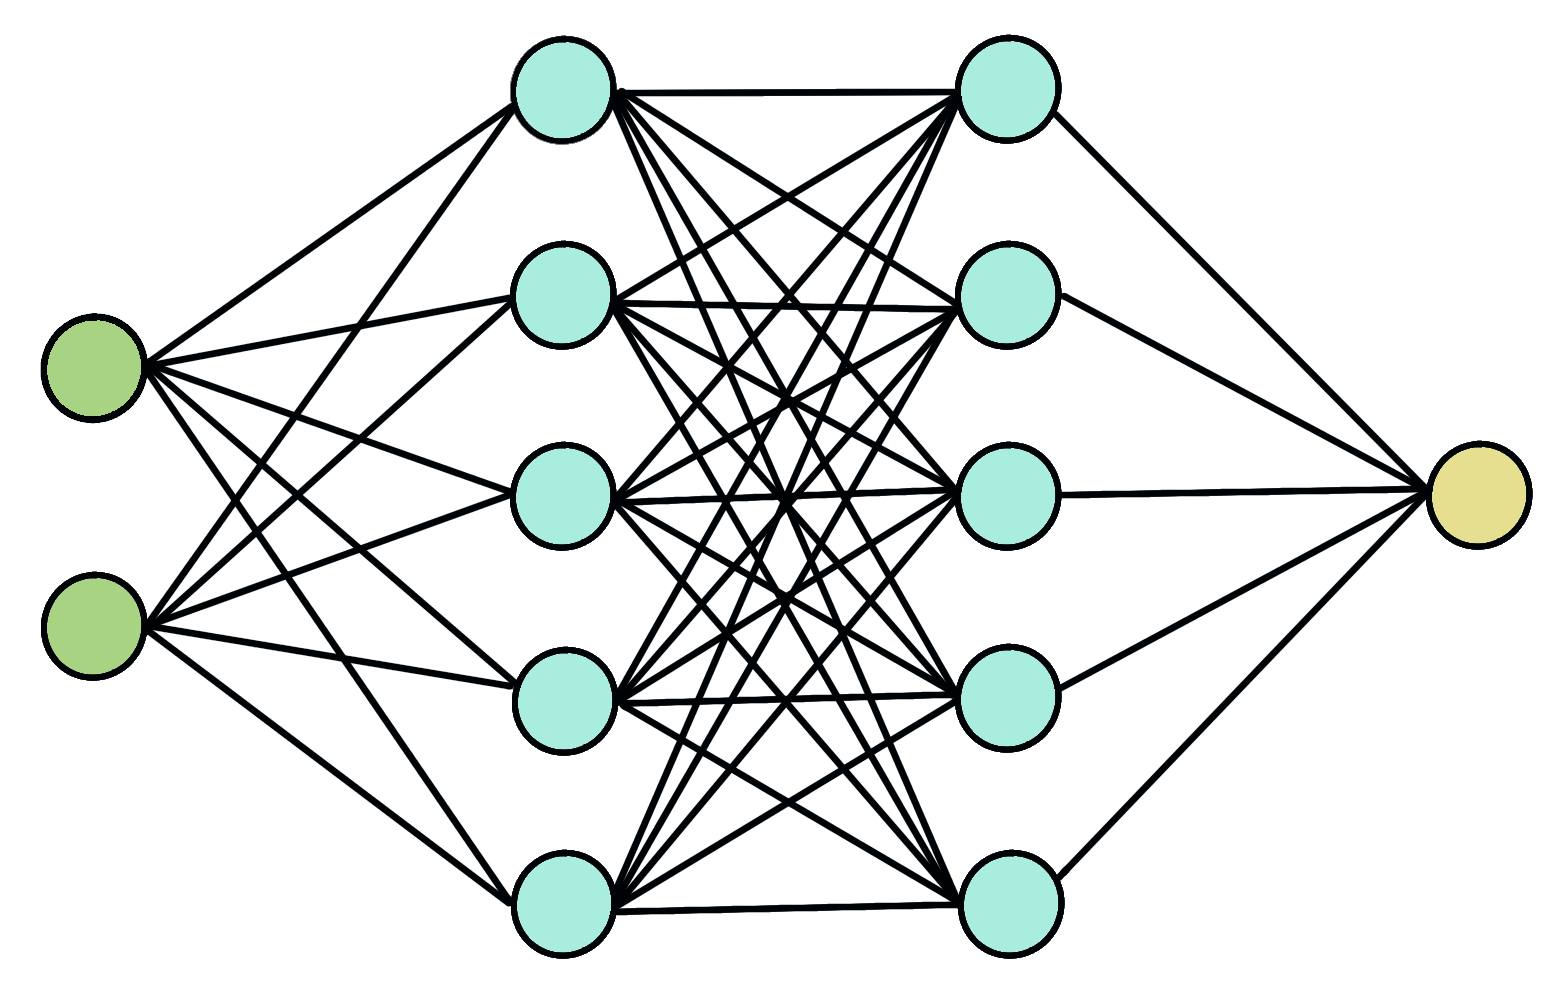
\includegraphics[width=3cm]{network.png}};
            \node at (8.5,0.35) {\large \textbf{Parametric PINN}};

            \draw[->, black, line width=2pt] (10.5,1.25) -- (11.5,1.25);

            \draw[draw=black,dashed] (12,0) rectangle ++ (5,2.5);	
            \node at (14.5,1.85) {\Large \textbf{Output}};
            \node at (14.5,1.1) {\large $u_\theta$ : prediction of};
            \node at (14.5,0.5) {\large the PDE solution $u$};
        \end{tikzpicture}
    \end{tcolorbox}
\end{document}